\section{Determination of e-beam exposed PMMA vertex mobilities}

Obtained PMMA viscosity profile couldn't be used for thermal reflow simulation so far -- the analytical approach based on profile Fourier transform could be applied in case of uniform viscosity only.
On the other hand, the numerical approach allows reflow simulation of non-uniform structures, but it bases on vertex mobilities, not viscosity.
Therefore, one should investigate the correlation between polymer viscosity and vertex mobilities of its surface.
For this purpose, thermal reflow was simulated by both approaches for the PMMA rectangular gratings, which parameters corresponded to Leveder study~\cite{Leveder_2010} -- 2 $\mu$m pitch and 28 nm depth.
First, for PMMA viscosity values in range 10$^2$--10$^6$ Pa$\cdot$s grating reflow was simulated analytically with constant time steps.
Then the grating surface was reconstructed in SE and surface evolution during grating reflow was simulated numerically with vertex mobility equal to 1.
During the numerical simulation, \textit{scale} values giving the same grating profiles as ones obtained using analytical approach, were determined (Fig.~\ref{fig:gratings_reflow}).
It was found that in the beginning of reflow there is a slight discrepancy between profiles simulated analytically and numerically but then both approaches lead to almost sinusoidal shape as it is predicted by equations~\ref{eq:Fourier_1},~\ref{eq:Fourier_2}~and~\ref{eq:Fourier_3}.
Time-\textit{scale} data obtained for different viscosity values showed almost direct proportionality between \textit{scale} and time ($t$) (Fig.~\ref{fig:alphas}):
\begin{equation} \label{eq:scale_alpha_t}
	scale \approx \alpha \cdot t.
\end{equation}
The values of $\alpha$ obtained by approximation of $t$-\textit{scale} data by a function~\ref{eq:scale_alpha_t} demonstrated quite linear dependence of $\ln(\alpha)$ on $\ln(\eta)$ (Fig.~\ref{fig:final_fit}).
The approximation of $\ln(\eta)$-$\ln(\alpha)$ data by the function
\begin{equation}
	\alpha = \frac{C}{\eta^\beta}
\end{equation}
resulted in $C$ and $\beta$ values equal to 26.142 and 0.989.
Thus, there is almost inverse proportionality between $\alpha$ and polymer viscosity:
\begin{equation}
	\alpha \approx \frac{26.142}{\eta}.
\end{equation}

\begin{figure}[h]
	\centering
	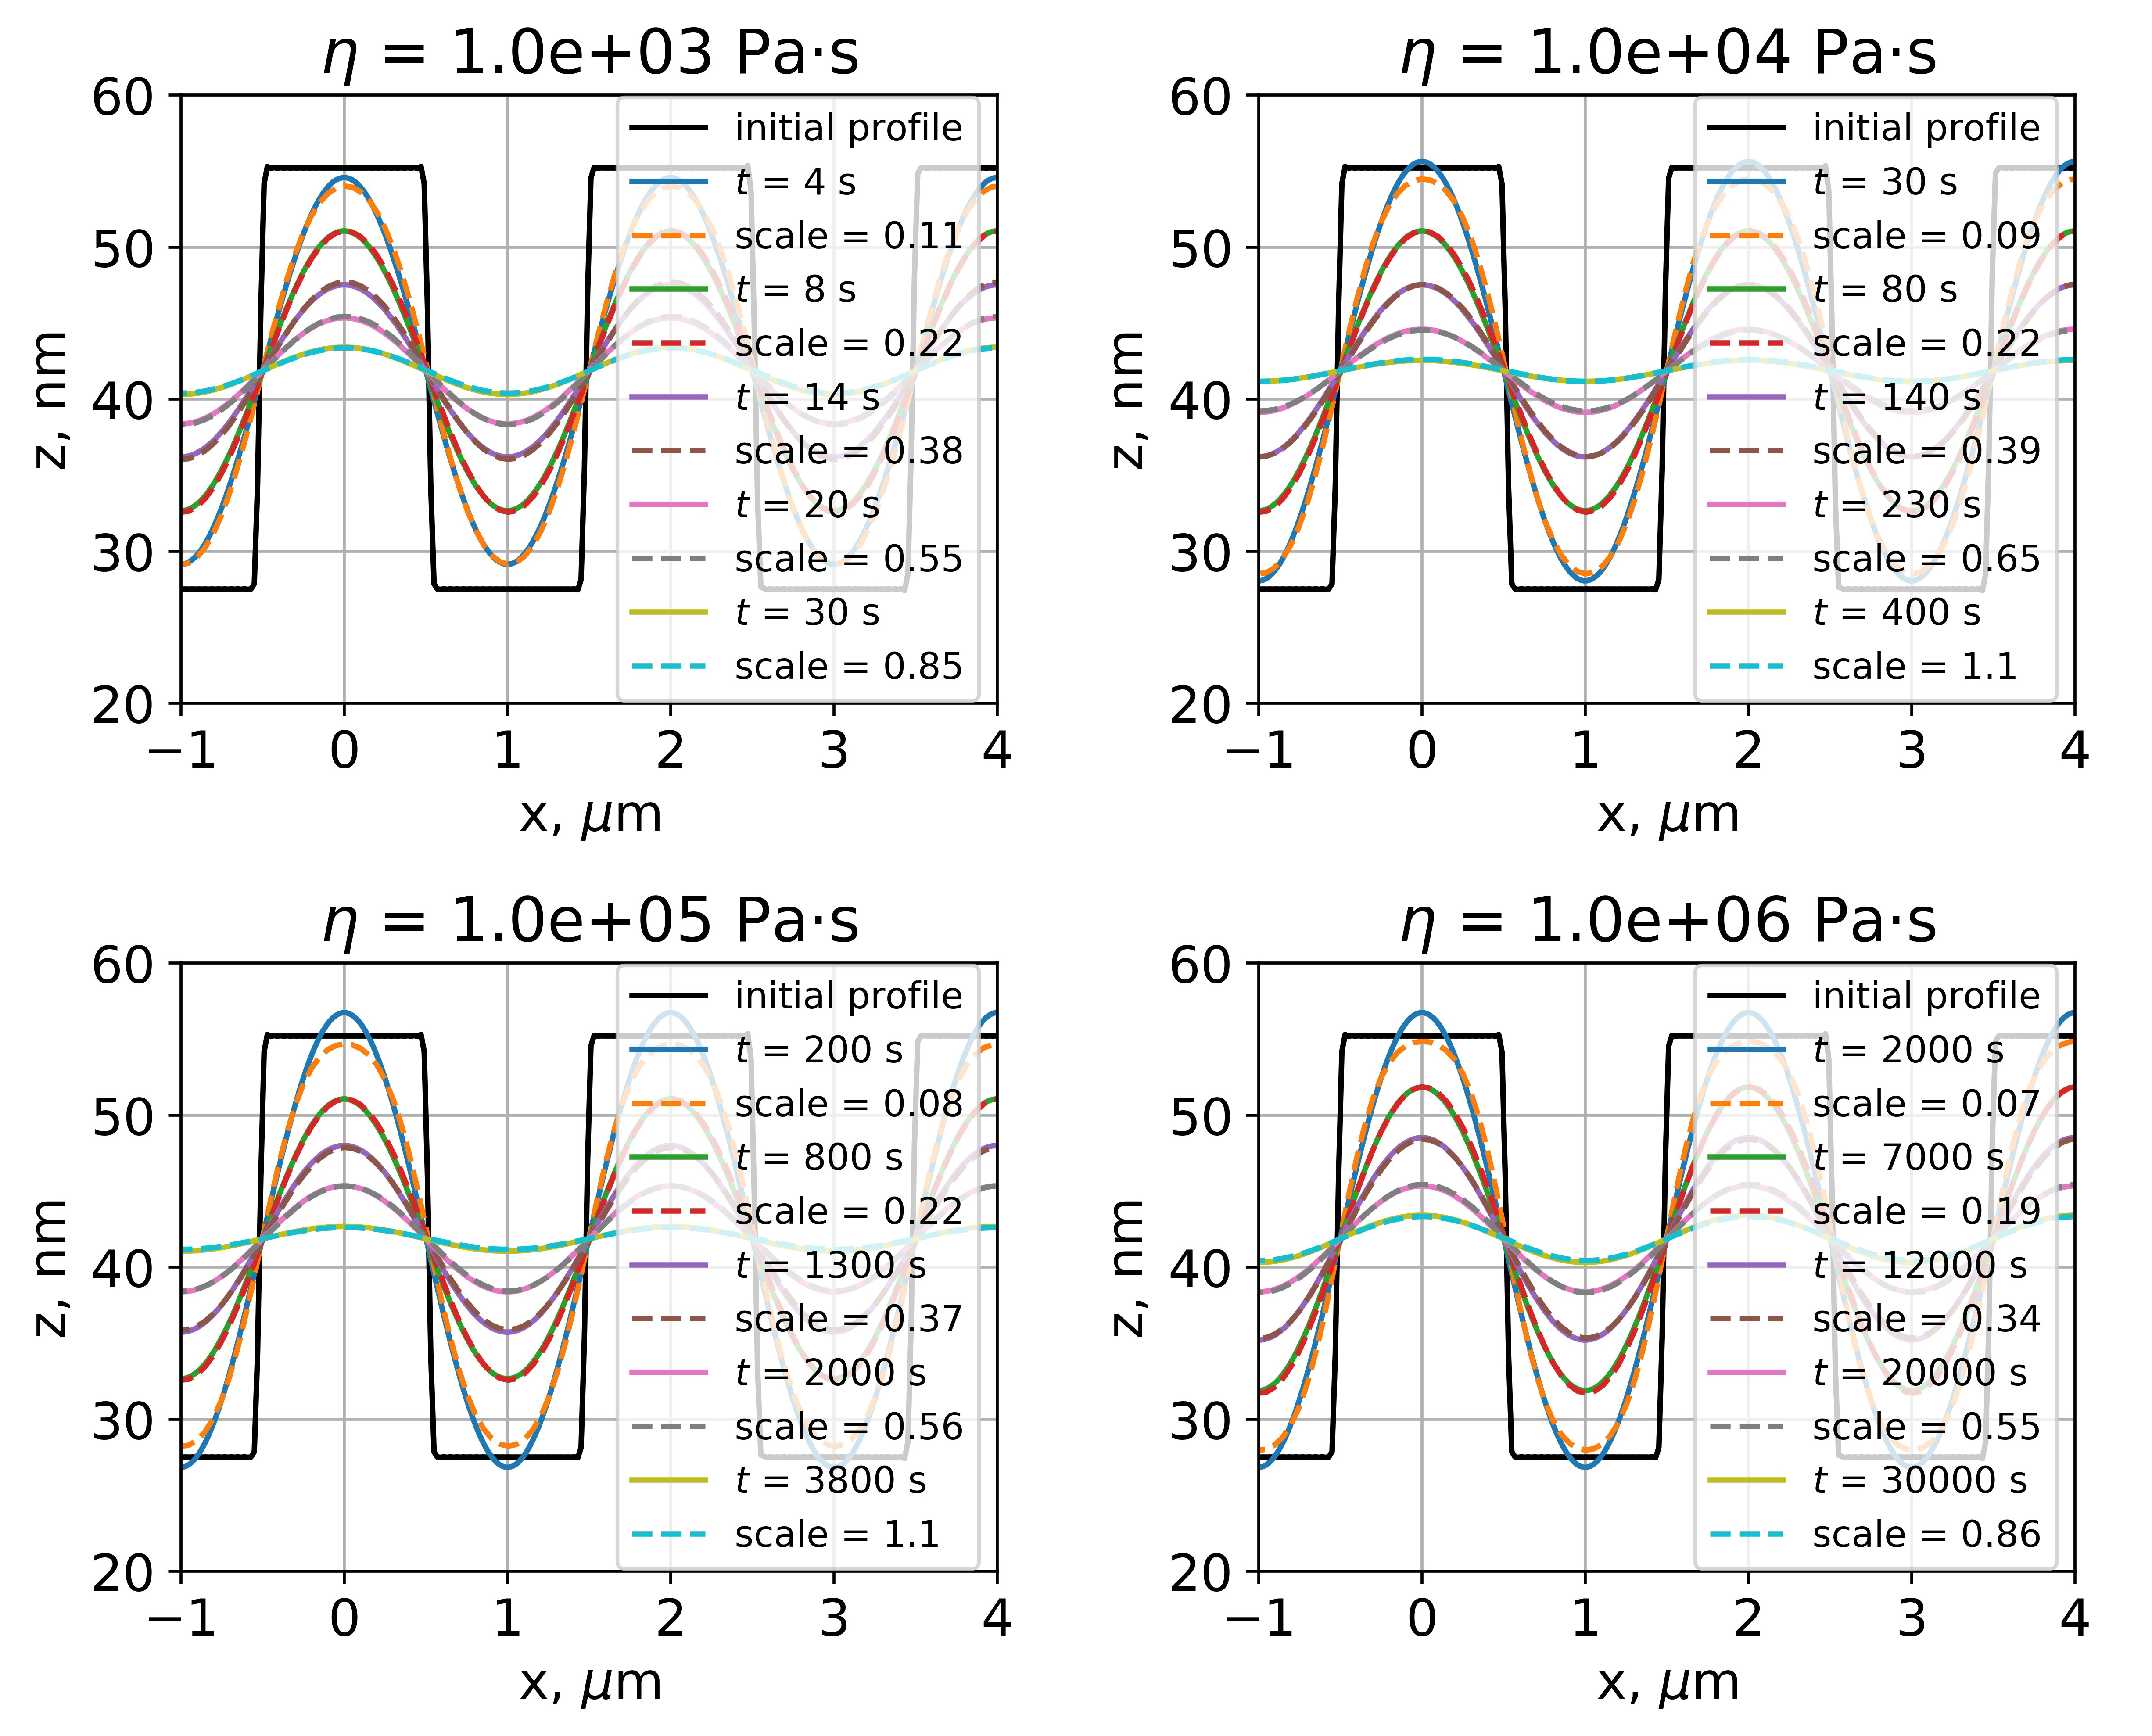
\includegraphics[width=\linewidth]{gratings_reflow}
	\caption{Thermal reflow of PMMA rectangular grating simulated by analytical and numerical approaches for different PMMA viscosity values.}
	\label{fig:gratings_reflow}
\end{figure}

\begin{figure}[h]
	\centering
	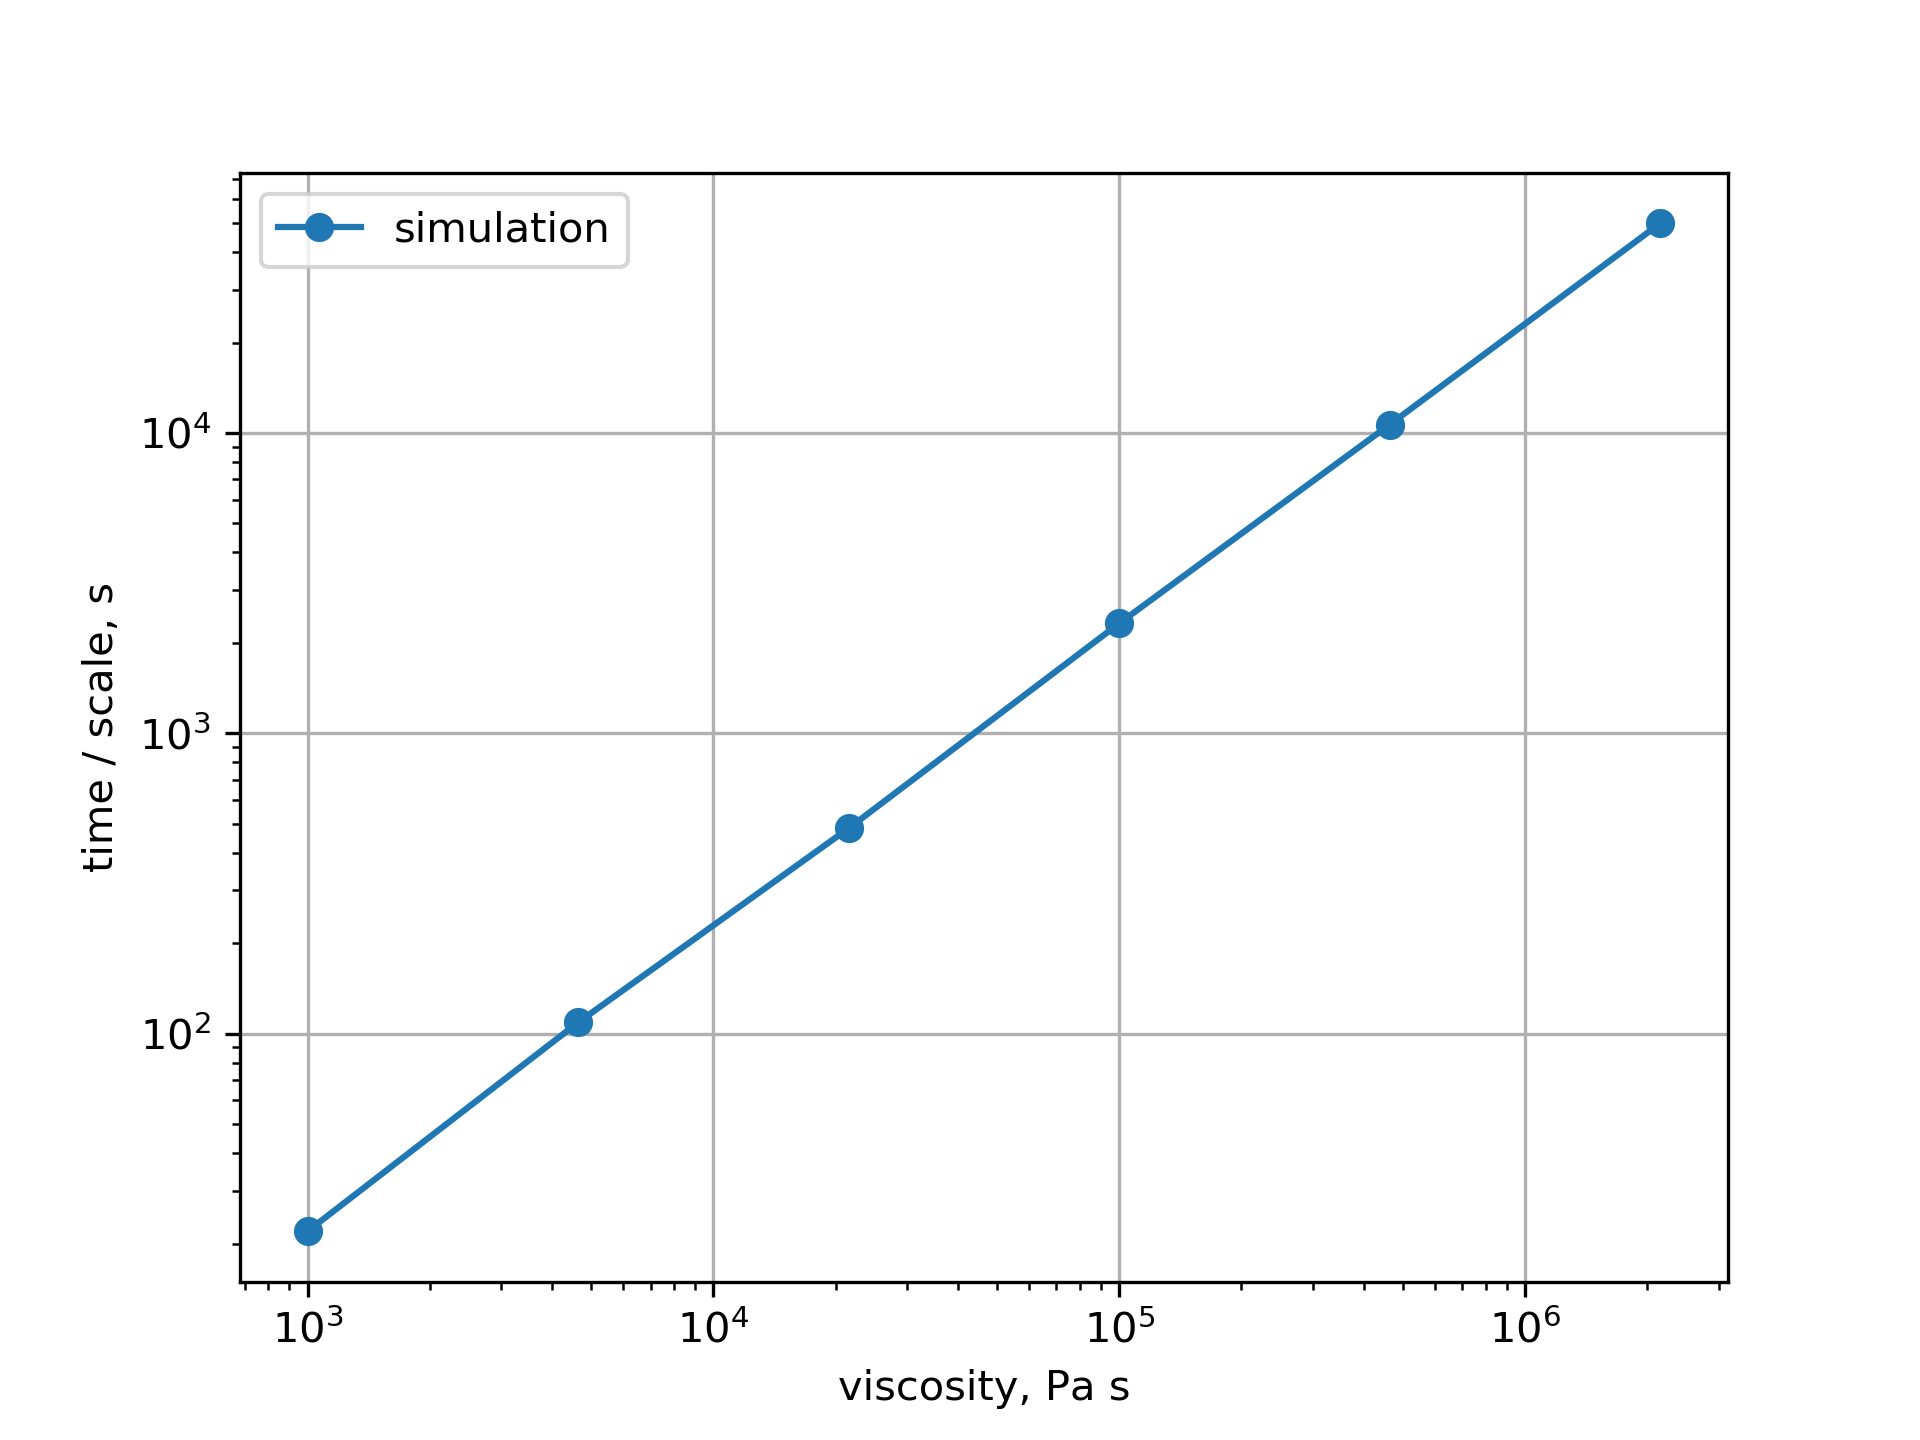
\includegraphics[width=\linewidth]{alphas} \\
	\caption{Time-\textit{scale} dependencies for different viscosity values fitted with linear function.}
	\label{fig:alphas}
\end{figure}

\begin{figure}
	\centering
	\includegraphics[width=0.6\linewidth]{С_gamma}
	\vspace{-1em}
	\caption{Linear fit of obtained $\ln(\alpha)$-$\ln(\eta)$ data.}
	\label{fig:final_fit}
\end{figure}

The determined relation between PMMA viscosity and $\alpha$ (which represents the ratio of $scale$ to $t$) enables mobility-based thermal reflow simulation by SE.
The point is that SE allows to monitor $scale$ value during the simulation, but originally $scale$ is not equal to reflow time.
The most convenient relation between $scale$ and time would be an equality ($scale \equiv t$) and it could be achieved by setting mobility equal to $\alpha$.
Indeed, if one simultaneously set
\begin{equation} \label{eq:mu_scale}
	\cases{\mu \equiv \alpha = \frac{scale}{t}, & \\
		scale = t &}
\end{equation}
the equation~\ref{eq:SE_v} doesn't change:
\begin{equation}
	\vec{\delta} = \frac{\vec{F}}{A/3} \cdot \frac{scale}{t} \cdot t \equiv \frac{\vec{F}}{A/3} \cdot scale.
\end{equation}

The equations~\ref{eq:mu_scale} is the final piece in mobility-based thermal reflow simulation of e-beam exposed PMMA.
Viscosity profile of PMMA, obtained at previous step could be easily converted into mobility profile using formula (Fig.~\ref{fig:mob_arr})
\begin{equation} \label{eq:mu_eta}
	\mu = \frac{26.142}{\eta}.
\end{equation}
Thus, one can reconstruct the surface of PMMA structure in SE, set proper mobilities of surface vertices and then run SE simulation with tracking the $scale$ factor, which will be exactly equal to reflow time.

\begin{figure}[h]
	\centering
	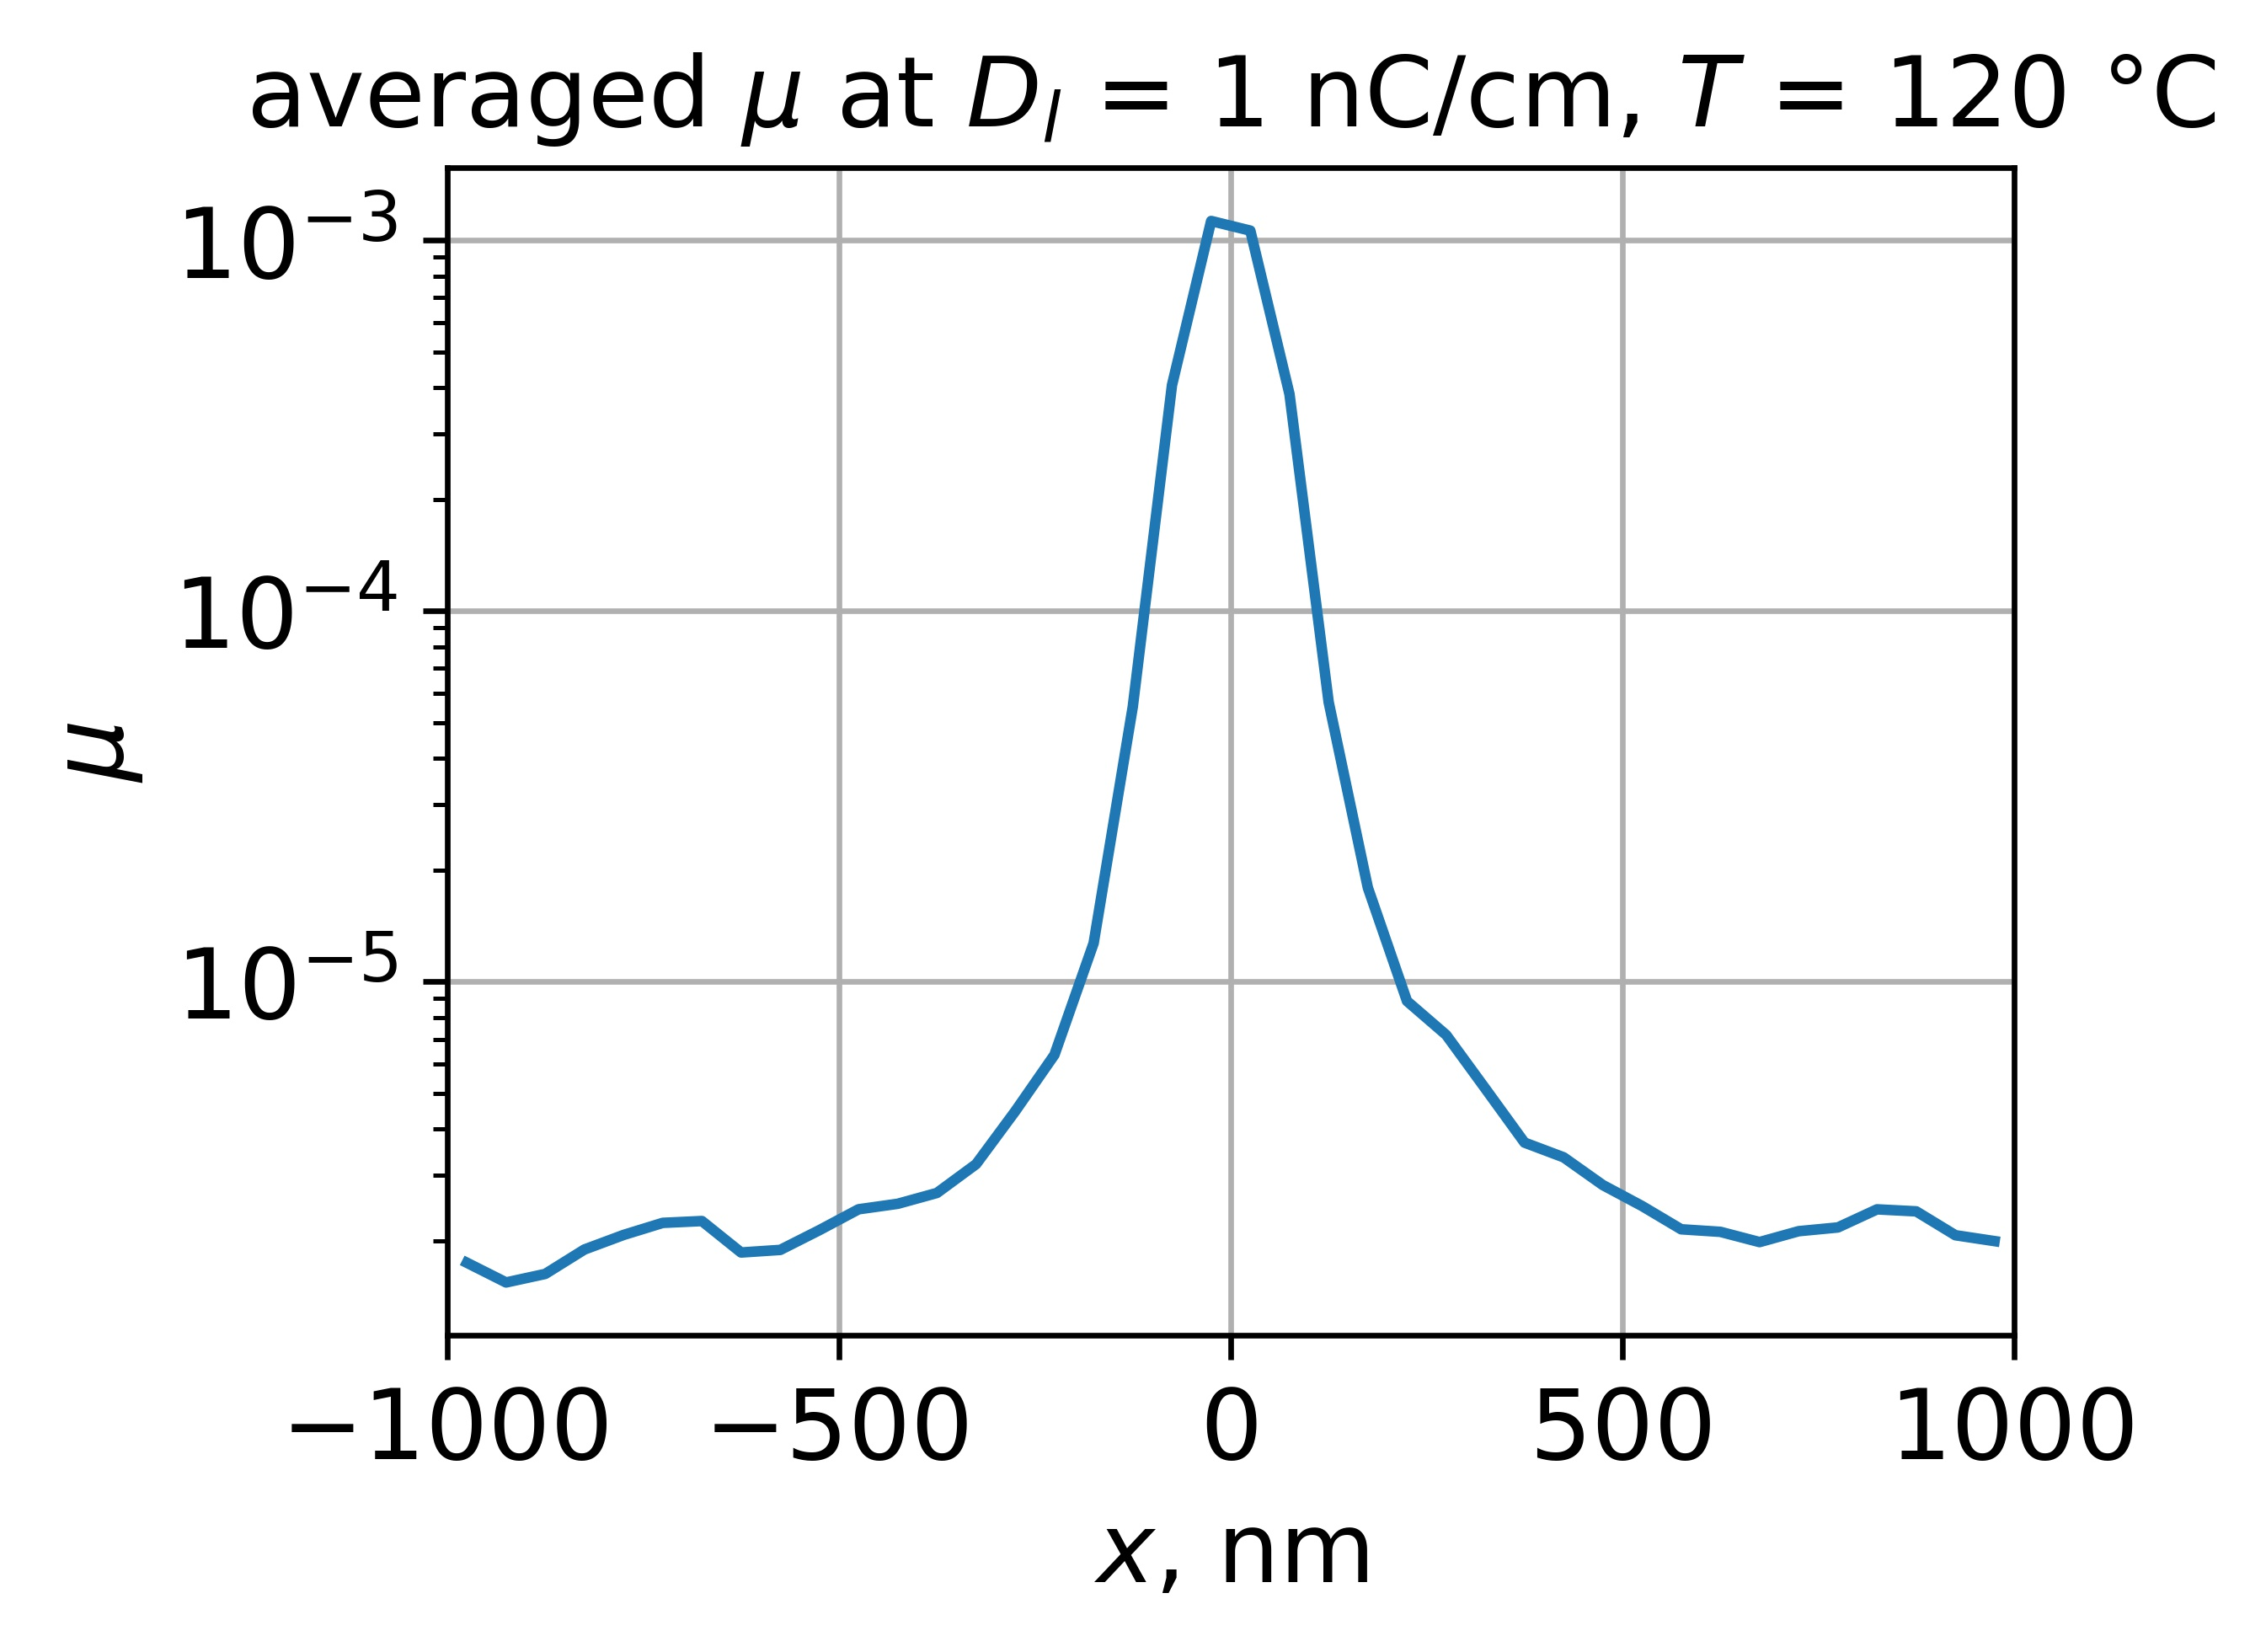
\includegraphics[width=0.6\linewidth]{mob_arr_1_nC_cm_120C_LOG}
	\vspace{-1em}
	\caption{
		Simulation of averaged (along $z$ axis) vertex mobility profile of e-beam exposed PMMA layer for 120 $^\circ$C.
		Line dose is 1 nC/cm, e-beam energy -- 20 keV, PMMA layer thickness -- 500 nm.
		Initial PMMA number average molecular weight is 271000.
	}
	\label{fig:mob_arr}
\end{figure}
